\documentclass[]{article}
\usepackage{lmodern}
\usepackage{amssymb,amsmath}
\usepackage{ifxetex,ifluatex}
\usepackage{fixltx2e} % provides \textsubscript
\ifnum 0\ifxetex 1\fi\ifluatex 1\fi=0 % if pdftex
  \usepackage[T1]{fontenc}
  \usepackage[utf8]{inputenc}
\else % if luatex or xelatex
  \ifxetex
    \usepackage{mathspec}
  \else
    \usepackage{fontspec}
  \fi
  \defaultfontfeatures{Ligatures=TeX,Scale=MatchLowercase}
\fi
% use upquote if available, for straight quotes in verbatim environments
\IfFileExists{upquote.sty}{\usepackage{upquote}}{}
% use microtype if available
\IfFileExists{microtype.sty}{%
\usepackage{microtype}
\UseMicrotypeSet[protrusion]{basicmath} % disable protrusion for tt fonts
}{}
\usepackage[margin=1in]{geometry}
\usepackage{hyperref}
\hypersetup{unicode=true,
            pdftitle={Exercise Sheet 2, 2019},
            pdfauthor={Gent Rexha (11832486), Princ Mullatahiri (11846033)},
            pdfborder={0 0 0},
            breaklinks=true}
\urlstyle{same}  % don't use monospace font for urls
\usepackage{color}
\usepackage{fancyvrb}
\newcommand{\VerbBar}{|}
\newcommand{\VERB}{\Verb[commandchars=\\\{\}]}
\DefineVerbatimEnvironment{Highlighting}{Verbatim}{commandchars=\\\{\}}
% Add ',fontsize=\small' for more characters per line
\usepackage{framed}
\definecolor{shadecolor}{RGB}{248,248,248}
\newenvironment{Shaded}{\begin{snugshade}}{\end{snugshade}}
\newcommand{\AlertTok}[1]{\textcolor[rgb]{0.94,0.16,0.16}{#1}}
\newcommand{\AnnotationTok}[1]{\textcolor[rgb]{0.56,0.35,0.01}{\textbf{\textit{#1}}}}
\newcommand{\AttributeTok}[1]{\textcolor[rgb]{0.77,0.63,0.00}{#1}}
\newcommand{\BaseNTok}[1]{\textcolor[rgb]{0.00,0.00,0.81}{#1}}
\newcommand{\BuiltInTok}[1]{#1}
\newcommand{\CharTok}[1]{\textcolor[rgb]{0.31,0.60,0.02}{#1}}
\newcommand{\CommentTok}[1]{\textcolor[rgb]{0.56,0.35,0.01}{\textit{#1}}}
\newcommand{\CommentVarTok}[1]{\textcolor[rgb]{0.56,0.35,0.01}{\textbf{\textit{#1}}}}
\newcommand{\ConstantTok}[1]{\textcolor[rgb]{0.00,0.00,0.00}{#1}}
\newcommand{\ControlFlowTok}[1]{\textcolor[rgb]{0.13,0.29,0.53}{\textbf{#1}}}
\newcommand{\DataTypeTok}[1]{\textcolor[rgb]{0.13,0.29,0.53}{#1}}
\newcommand{\DecValTok}[1]{\textcolor[rgb]{0.00,0.00,0.81}{#1}}
\newcommand{\DocumentationTok}[1]{\textcolor[rgb]{0.56,0.35,0.01}{\textbf{\textit{#1}}}}
\newcommand{\ErrorTok}[1]{\textcolor[rgb]{0.64,0.00,0.00}{\textbf{#1}}}
\newcommand{\ExtensionTok}[1]{#1}
\newcommand{\FloatTok}[1]{\textcolor[rgb]{0.00,0.00,0.81}{#1}}
\newcommand{\FunctionTok}[1]{\textcolor[rgb]{0.00,0.00,0.00}{#1}}
\newcommand{\ImportTok}[1]{#1}
\newcommand{\InformationTok}[1]{\textcolor[rgb]{0.56,0.35,0.01}{\textbf{\textit{#1}}}}
\newcommand{\KeywordTok}[1]{\textcolor[rgb]{0.13,0.29,0.53}{\textbf{#1}}}
\newcommand{\NormalTok}[1]{#1}
\newcommand{\OperatorTok}[1]{\textcolor[rgb]{0.81,0.36,0.00}{\textbf{#1}}}
\newcommand{\OtherTok}[1]{\textcolor[rgb]{0.56,0.35,0.01}{#1}}
\newcommand{\PreprocessorTok}[1]{\textcolor[rgb]{0.56,0.35,0.01}{\textit{#1}}}
\newcommand{\RegionMarkerTok}[1]{#1}
\newcommand{\SpecialCharTok}[1]{\textcolor[rgb]{0.00,0.00,0.00}{#1}}
\newcommand{\SpecialStringTok}[1]{\textcolor[rgb]{0.31,0.60,0.02}{#1}}
\newcommand{\StringTok}[1]{\textcolor[rgb]{0.31,0.60,0.02}{#1}}
\newcommand{\VariableTok}[1]{\textcolor[rgb]{0.00,0.00,0.00}{#1}}
\newcommand{\VerbatimStringTok}[1]{\textcolor[rgb]{0.31,0.60,0.02}{#1}}
\newcommand{\WarningTok}[1]{\textcolor[rgb]{0.56,0.35,0.01}{\textbf{\textit{#1}}}}
\usepackage{graphicx,grffile}
\makeatletter
\def\maxwidth{\ifdim\Gin@nat@width>\linewidth\linewidth\else\Gin@nat@width\fi}
\def\maxheight{\ifdim\Gin@nat@height>\textheight\textheight\else\Gin@nat@height\fi}
\makeatother
% Scale images if necessary, so that they will not overflow the page
% margins by default, and it is still possible to overwrite the defaults
% using explicit options in \includegraphics[width, height, ...]{}
\setkeys{Gin}{width=\maxwidth,height=\maxheight,keepaspectratio}
\IfFileExists{parskip.sty}{%
\usepackage{parskip}
}{% else
\setlength{\parindent}{0pt}
\setlength{\parskip}{6pt plus 2pt minus 1pt}
}
\setlength{\emergencystretch}{3em}  % prevent overfull lines
\providecommand{\tightlist}{%
  \setlength{\itemsep}{0pt}\setlength{\parskip}{0pt}}
\setcounter{secnumdepth}{0}
% Redefines (sub)paragraphs to behave more like sections
\ifx\paragraph\undefined\else
\let\oldparagraph\paragraph
\renewcommand{\paragraph}[1]{\oldparagraph{#1}\mbox{}}
\fi
\ifx\subparagraph\undefined\else
\let\oldsubparagraph\subparagraph
\renewcommand{\subparagraph}[1]{\oldsubparagraph{#1}\mbox{}}
\fi

%%% Use protect on footnotes to avoid problems with footnotes in titles
\let\rmarkdownfootnote\footnote%
\def\footnote{\protect\rmarkdownfootnote}

%%% Change title format to be more compact
\usepackage{titling}

% Create subtitle command for use in maketitle
\providecommand{\subtitle}[1]{
  \posttitle{
    \begin{center}\large#1\end{center}
    }
}

\setlength{\droptitle}{-2em}

  \title{Exercise Sheet 2, 2019}
    \pretitle{\vspace{\droptitle}\centering\huge}
  \posttitle{\par}
  \subtitle{6.0 VU Advanced Database Systems}
  \author{Gent Rexha (11832486), Princ Mullatahiri (11846033)}
    \preauthor{\centering\large\emph}
  \postauthor{\par}
      \predate{\centering\large\emph}
  \postdate{\par}
    \date{08.05.2019}


\begin{document}
\maketitle

\hypertarget{exercise-1-mapreduce-4-punkte}{%
\subsection{Exercise 1 (MapReduce) {[}4
Punkte{]}}\label{exercise-1-mapreduce-4-punkte}}

\textbf{a)} First of all, we take the input and map the author to the
row in the \texttt{checkouts-by-title.csv} file
\textless{}Author,Row\textgreater{}. After that most of the heavy
lifting takes place in the reducer, where a hashmap of all the titles of
the current creator is created and for each value in our values list the
number of checkouts is updated for the corresponding title. After having
iterated all the values, the title with the maximum amount of checkouts
is written out with it's corresponding author.

Statistics:

\begin{itemize}
\tightlist
\item
  replication rate = ???
\item
  input size = 6789 Mbyte
\item
  output = 27 Mbyte
\end{itemize}

\begin{figure}[h]

{\centering 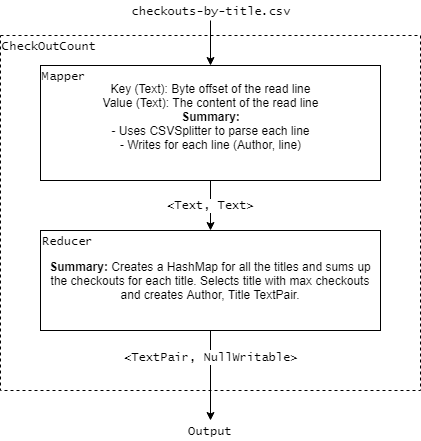
\includegraphics[width=300px]{images/Exercise_1_Task_A} 

}

\caption{\label{fig:figs}Diagram of the Map Reduce job to solve Task A}\label{fig:unnamed-chunk-1}
\end{figure}

\textbf{b)} For this task we used the MultipleInputs class. It allows
you to create MapReduce jobs with multiple mapper functions, each for a
different input file. The results of the mappers is then sent to the
same reducer function. For the two datasets we've created two separate
mappers which send the row with the author as key to the reducer. The
reducer then creates two HashMaps, for both checkouts and inventory.
Checkout HashMap includes all the titles and sums up the checkouts for
each title. After that it selects the title with max checkouts and
creates Author, Title TextPair and adds PublicationYear, Subjects,
ItemLocation from the second HashMap where all the locations for all
titles of said Author are stored.

Statistics:

\begin{itemize}
\tightlist
\item
  replication rate = ???
\item
  input = 13944 Mbyte
\item
  output = 36 Mbyte
\end{itemize}

\begin{figure}[h]

{\centering 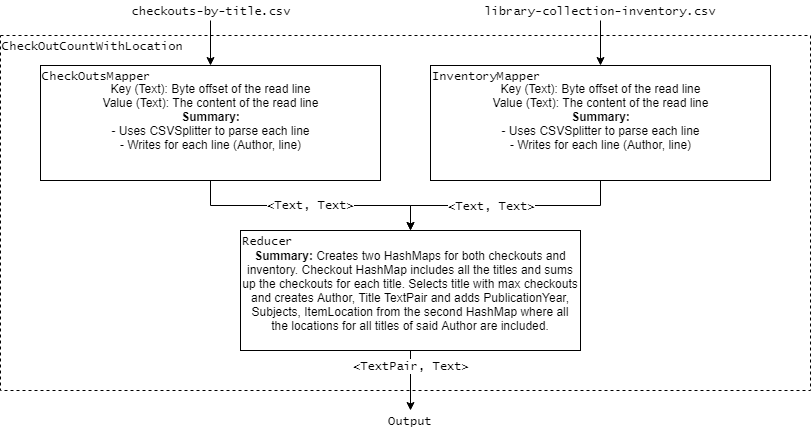
\includegraphics[width=450px]{images/Exercise_1_Task_B} 

}

\caption{\label{fig:figs}Diagram of the Map Reduce job to solve Task B}\label{fig:unnamed-chunk-2}
\end{figure}

\newpage

\hypertarget{exercise-2-costs-of-mapreduce-1-punkte}{%
\subsection{Exercise 2 (Costs of MapReduce) {[}1
Punkte{]}}\label{exercise-2-costs-of-mapreduce-1-punkte}}

\textbf{a)} In the Reducer, if not using a combiner, there is some skew
to be expected, given that different keys can receive different amounts
of values, resulting in different processing times. Key A can have many
values, for example, but key B can have very few or none, resulting in
more calculation for key A values and therefore more processing time.
This is till dependent on the \texttt{key,value} data distribution,
because in the extreme case where all of your values are of the same
key, the number of reducers doesn't matter. In this case a custom
partitioner might make more sense.

\textbf{b)} Considering a small number of reducers, more randomized key
values are expected at different reducers and a more even distribution
of one key's intensive processing values. This also leads to less
parellesim and may take longer. If the number of reducers is increased,
the likelihood that only one reducer will end up with a \textless{}key,
value\textgreater{} pair where many values are also higher. Therefore,
the skewedness is increased to a very important level. On the other
hand, a maximum of parallelism is achieved, but the problem of overhead
computing comes with this.

\textbf{c)} If we use a combiner in the WordCount MapReduce program then
we'd have less reducer calculation and more for mapping phase, basically
we'd calculate sum of word occurrences for each mapper node in a
document. And we don't expect to be a significant skew because reducer
would have less work to do. The best way to avoid skewing would be to
use combiner and partition where we determine which task reduction
receives which key and its values?list, to partition the key we could
use a hash function and this would ensure that all pairs with the same
key go to the same reducer.

\textbf{d)} Communication costs are made by the size of the input file,
the sum of the sizes of all files passed from the map process to reduce
processes and the sum of the output sizes of reducer processes, so
basically it does not depend on the number of reducers we have, because
even if we have 1 reducer or if we have 100000 reducers, we would still
have the same size of the input file. We'd still have the same file size
input, the same sum of all file sizes passed from map to reduce, and the
sum of all reducer outputs.

\newpage

\hypertarget{exercise-3-relational-operations-2-punkte}{%
\subsection{Exercise 3 (Relational Operations) {[}2
Punkte{]}}\label{exercise-3-relational-operations-2-punkte}}

\begin{figure}[h]

{\centering 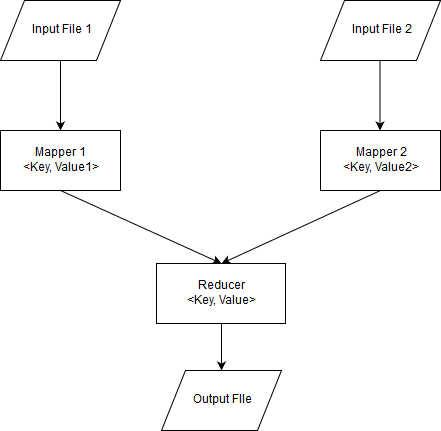
\includegraphics[width=300px]{images/Exercise3} 

}

\caption{\label{fig:figs}Mapreduce Sketch for Bag Union and Difference}\label{fig:unnamed-chunk-3}
\end{figure}

\textbf{a)} Bag Union Pseudo-code:

\begin{Shaded}
\begin{Highlighting}[]
\NormalTok{sum =}\StringTok{ }\DecValTok{0}
\NormalTok{foreach val}\OperatorTok{:}\NormalTok{value }
\NormalTok{    sum =}\StringTok{ }\NormalTok{sum }\OperatorTok{+}\StringTok{ }\DecValTok{1}
\KeywordTok{context.write}\NormalTok{(Key, sum)}
\end{Highlighting}
\end{Shaded}

First we get all values from the same key in reducer, then we iterate
through each value and increment sum variable, then we simply write to
output key and sum as value.

\textbf{b)} Bag Difference Pseudo-code:

\begin{Shaded}
\begin{Highlighting}[]
\NormalTok{first group by table origin and seperate them }\ControlFlowTok{in}\NormalTok{ diffrent vales }\OperatorTok{:}\StringTok{ }\NormalTok{value }\DecValTok{1}\NormalTok{ and }
\NormalTok{value }\DecValTok{2}\NormalTok{ corresponding to input file }\DecValTok{1}\NormalTok{ and input file }\DecValTok{2}
\NormalTok{sum_value1 =}\StringTok{ }\DecValTok{0}
\NormalTok{sum_value2 =}\StringTok{ }\DecValTok{0}
\NormalTok{foreach val}\OperatorTok{:}\StringTok{ }\NormalTok{value }\DecValTok{1}
\NormalTok{    sum_value1 =}\StringTok{ }\NormalTok{sum_value1 }\OperatorTok{+}\StringTok{ }\DecValTok{1}
\NormalTok{foreach val}\OperatorTok{:}\StringTok{ }\NormalTok{value }\DecValTok{2}
\NormalTok{    sum_value2 =}\StringTok{ }\NormalTok{sum_value2 }\OperatorTok{+}\StringTok{ }\DecValTok{1}

\ControlFlowTok{if}\NormalTok{ sum_value1 }\OperatorTok{>=}\StringTok{ }\NormalTok{sum_value2}
    \KeywordTok{context.write}\NormalTok{(Key, sum_value1 }\OperatorTok{-}\StringTok{ }\NormalTok{sum_value2)}
    
\NormalTok{First we group by table origin, then sum up values into two different variables sum_value1}
\NormalTok{and sum_value2, then we substract these values }\ControlFlowTok{if}\NormalTok{ value is positive, }
\NormalTok{we write to output }\ControlFlowTok{else}\NormalTok{ just skip that Key}

\NormalTok{dif =}\StringTok{ }\DecValTok{0}
\NormalTok{foreach val}\OperatorTok{:}\NormalTok{value }
\NormalTok{    sum =}\StringTok{ }\NormalTok{sum }\OperatorTok{+}\StringTok{ }\DecValTok{1}
\KeywordTok{context.write}\NormalTok{(Key, sum)}
\end{Highlighting}
\end{Shaded}

\newpage

\hypertarget{exercise-4-hive-exercise-4-punkte}{%
\subsection{Exercise 4 (Hive Exercise) {[}4
Punkte{]}}\label{exercise-4-hive-exercise-4-punkte}}

\textbf{a)} For task A we have to create tables and populate them with
data given in CSV files. So first we create the table, we tell that
values are seperated by comma and then give the location of CSV file.

\begin{verbatim}
CREATE EXTERNAL TABLE IF NOT EXISTS group11.badges (
id INT,class STRING, date DATE, name STRING, tagbased STRING, userid INT)
ROW FORMAT DELIMITED
FIELDS TERMINATED BY ','
STORED AS TEXTFILE
LOCATION '/home/adbs/2019S/shared/hive/badges.csv';
\end{verbatim}

\textbf{b)} Placeholder

\textbf{c)} Because Hive does not support subqueries and also does not
support unequal semi join we have to replace EXISTS with JOIN and then
filter the condition in where clause. And for count we place it in a
table and for filtering also call it in WHERE clause.

\begin{verbatim}
SELECT p.id
FROM comments c, badges_tmp b, 
posts p JOIN postlinks pl ON pl.postid = p.id,
users u, (SELECT COUNT(upvotes) as nrupvotes FROM users) k
WHERE c.postid=p.id 
AND u.upvotes + 3 >= k.nrupvotes
AND u.id=p.owneruserid 
AND pl.relatedpostid > p.id
AND u.creationdate = c.creationdate  
AND u.id = b.userid 
AND (b.name LIKE 'Autobiographer');
\end{verbatim}

\newpage

\hypertarget{exercise-5-spark-in-scala-4-punkte}{%
\subsection{Exercise 5 (Spark in Scala) {[}4
Punkte{]}}\label{exercise-5-spark-in-scala-4-punkte}}

\textbf{b)}

\begin{figure}[h]

{\centering 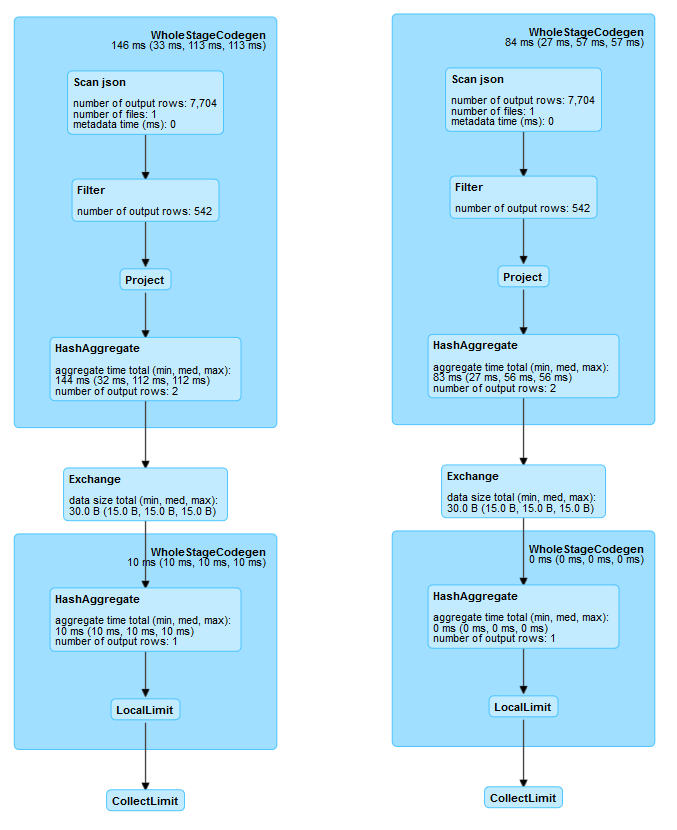
\includegraphics[width=300px]{images/query1} 

}

\caption{\label{fig:figs}LEFT: SQL DAG Diagram. RIGHT: Dataframe API DAG Diagram}\label{fig:unnamed-chunk-6}
\end{figure}

\begin{figure}[h]

{\centering 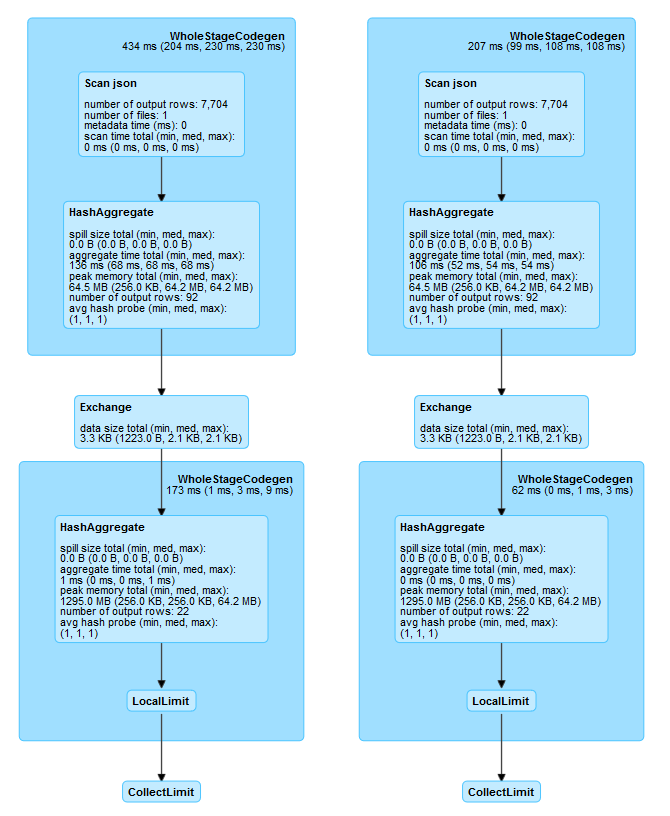
\includegraphics[width=300px]{images/query2} 

}

\caption{\label{fig:figs}LEFT: SQL DAG Diagram. RIGHT: Dataframe API DAG Diagram}\label{fig:unnamed-chunk-7}
\end{figure}

\begin{figure}[h]

{\centering 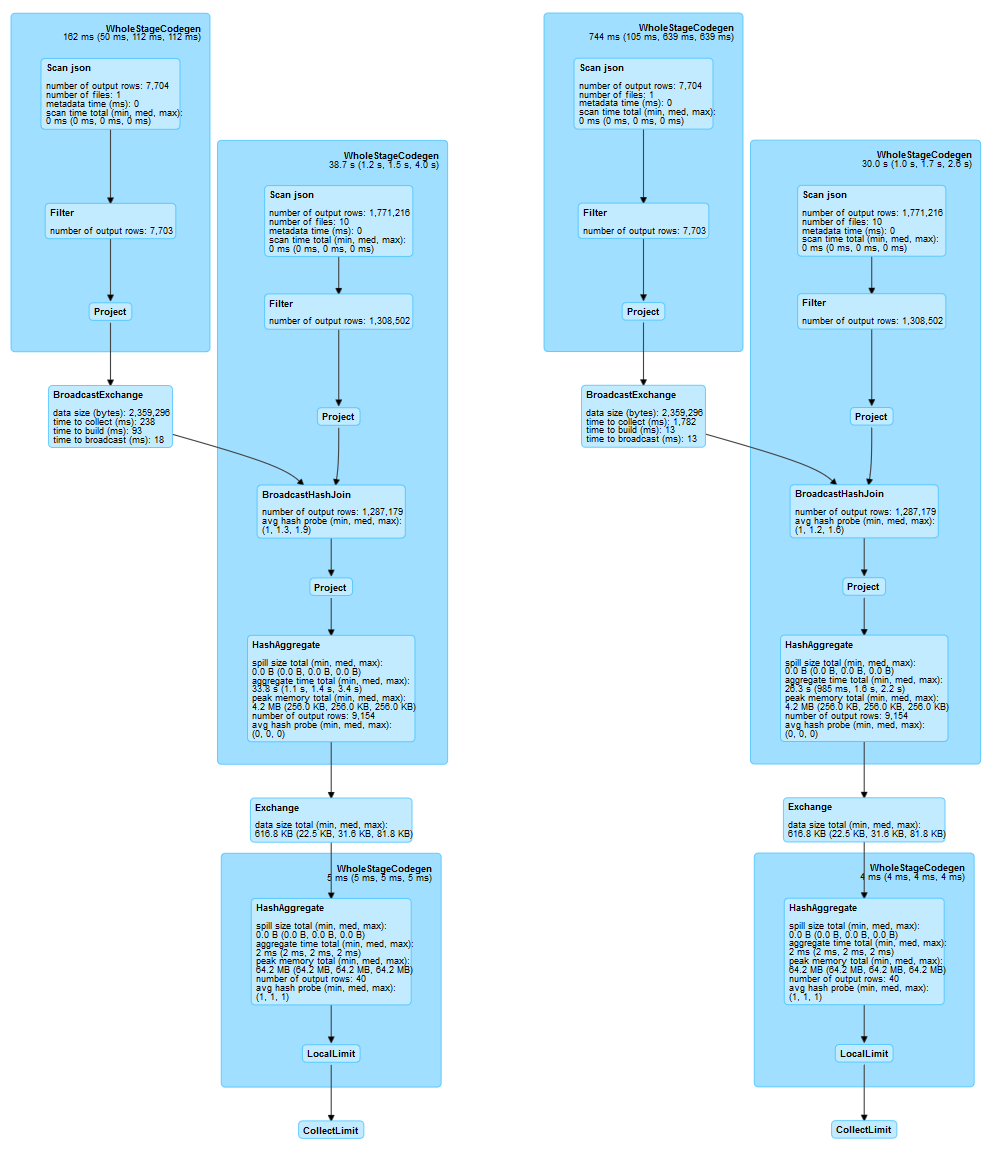
\includegraphics[width=300px]{images/query3} 

}

\caption{\label{fig:figs}LEFT: SQL DAG Diagram. RIGHT: Dataframe API DAG Diagram}\label{fig:unnamed-chunk-8}
\end{figure}

\begin{figure}[h]

{\centering 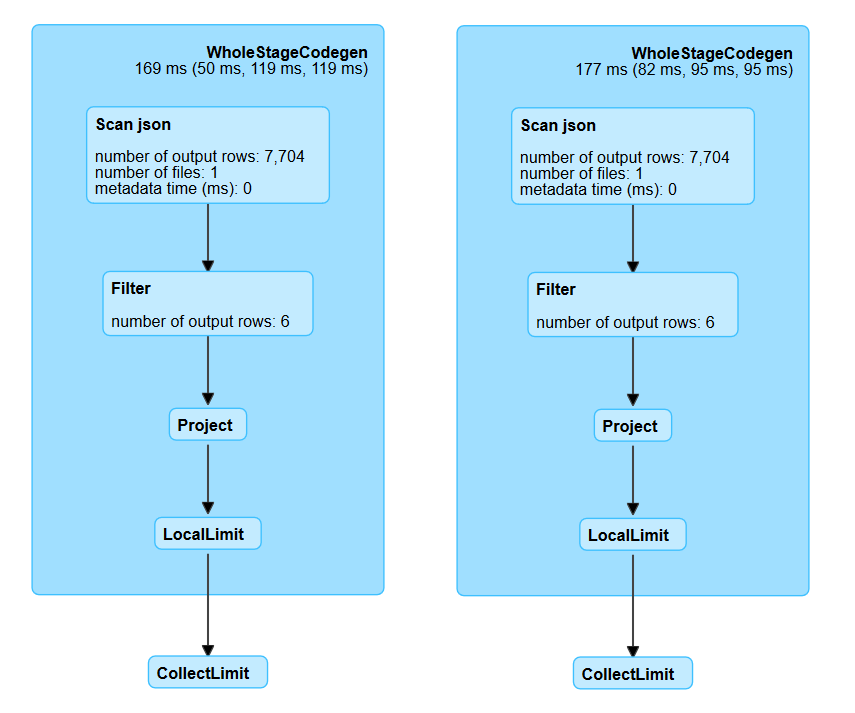
\includegraphics[width=300px]{images/query4} 

}

\caption{\label{fig:figs}LEFT: SQL DAG Diagram. RIGHT: Dataframe API DAG Diagram}\label{fig:unnamed-chunk-9}
\end{figure}

\begin{figure}[h]

{\centering 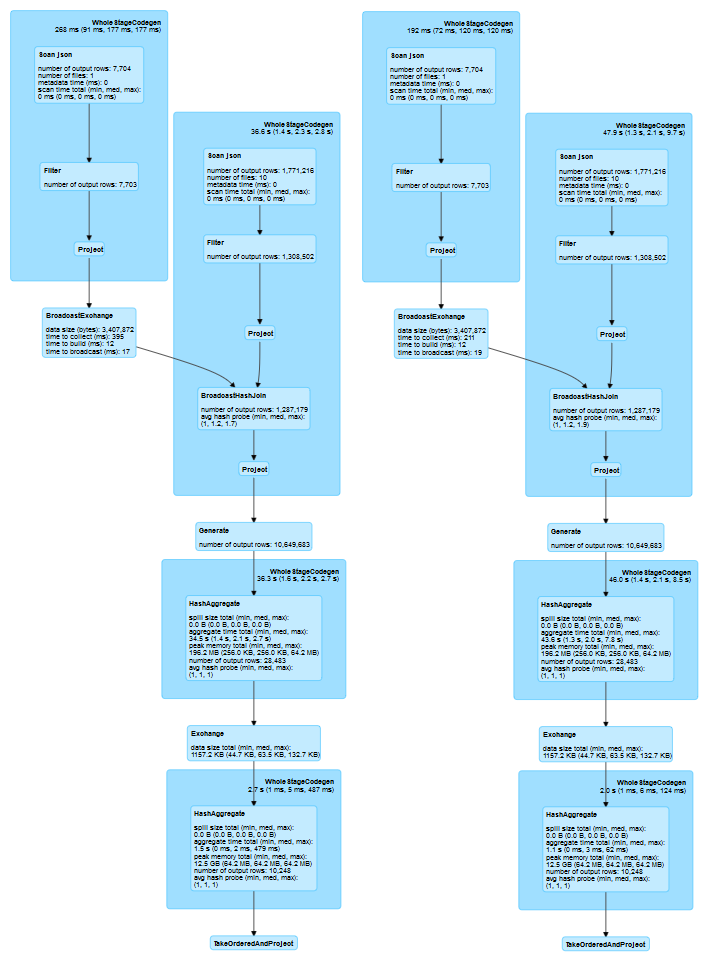
\includegraphics[width=300px]{images/query5} 

}

\caption{\label{fig:figs}LEFT: SQL DAG Diagram. RIGHT: Dataframe API DAG Diagram}\label{fig:unnamed-chunk-10}
\end{figure}

\begin{figure}[h]

{\centering 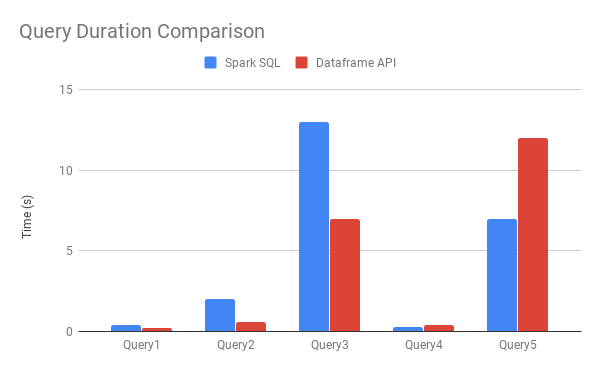
\includegraphics[width=300px]{images/Query Duration Comparison} 

}

\caption{\label{fig:figs}Query Duration Comparison}\label{fig:unnamed-chunk-11}
\end{figure}

\textbf{c)}

Narrow dependencies: Each partition of the parent RDD is used by at most
one partition of the child RDD.

\begin{verbatim}
[parent RDD partition] ---> [child RDD partition]
\end{verbatim}

Wide dependencies: Each partition of the parent RDD may be used by
multiple child partitions.

\begin{verbatim}
                       ---> [child RDD partition 1]
[parent RDD partition] ---> [child RDD partition 2]
                       ---> [child RDD partition 3]
\end{verbatim}

\begin{figure}[h]

{\centering 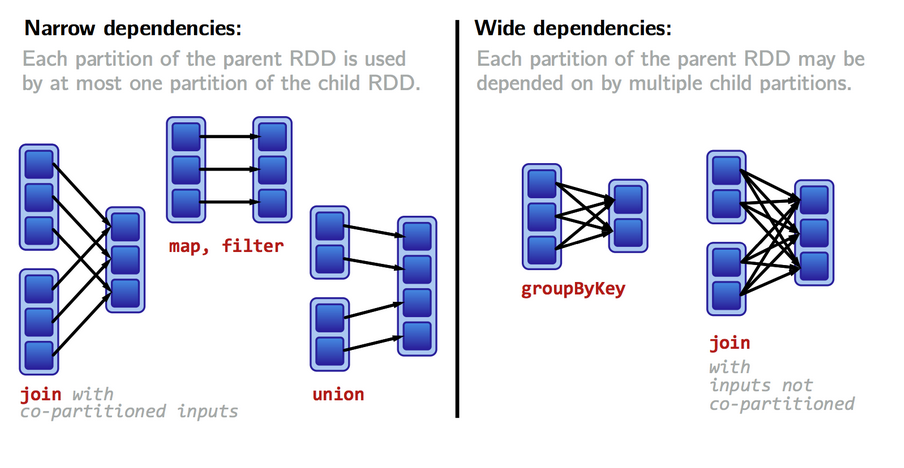
\includegraphics[width=300px]{images/Dependencies} 

}

\caption{\label{fig:figs}Wide and Narrow Dependencies Visualisation}\label{fig:unnamed-chunk-12}
\end{figure}


\end{document}
